\section{Navegação}
\label{sec:navegacao}

A navegação em campo aberto se torna um problema de tomada de decisões difícil,
devido à ausência de um mapa global atualizado, a falta de referenciais locais e
o excesso de ruído dos sensores, que produzem pouca informação válida para o
sistema. Apesar do veículo estar buscando um destino preestabelecido, dirigir-se
sempre em linha reta pode não ser a melhor decisão, ou mesmo impossível. Além
disto, a indicação da posição atual (localização) pode não ser totalmente
confiável.

Ainda que se utilize GPS, esse sistema apresenta erro na localização exata
(usualmente com um erro médio de cerca de 5
metros\foot{http://en.wikipedia.org/wiki/Error\_analysis\_for\_the\_Global\_Positioning\_System}),
pois considera-se também o fato de que o veículo não tem uma estrada ou via como
referência (ambiente não estruturado). Já no caso de dispositivos como o
odômetro, utilizados para manter um controle da localização por
\textit{dead-reckoning} \cite{Dudekbook}, a confiabilidade é ainda menor pois
há grande tendência de discrepância uma vez que o erro é cumulativo. Estas
discrepâncias podem ser resultantes de derrapagens das rodas, erros de estimação
da real distância percorrida ou mesmo das alterações involuntárias de direção do
veículo. Uma possível melhoria da precisão do GPS pode ser conseguida usando um
sistema de correção DGPS (GPS diferencial), onde antenas em solo são utilizadas
para aumentar a precisão do local estimado pelos sinais dos satélites. No
entanto, nem sempre este tipo de abordagem é possível pela falta desta
infraestrutura no local desejado, além de possuir um custo bem mais elevado em
relação a abordagem tradicional. No Brasil, o IBGE\foot{IBGE –
http://www.ibge.gov.br} disponibiliza serviços de posicionamento de precisão
através da RBMC\foot{RBMC –
http://www.ibge.gov.br/home/geociencias/geodesia/rbmc/rbmc.shtm} (Rede
Brasileira de Monitoramento Contínuo). O GPS tradicional possui um erro médio
usual entre 5 a 10 metros da posição estimada informada em relação a posição
real, enquanto um DGPS pode reduzir este erro médio para menos de 1 metro
(aproximadamente 50 cm).

É interessante observar que em aplicações de GPS em roteiros rodoviários (e
urbanos) a existência de um mapa local permite um certo ajuste de coerência que
visualmente dá a impressão de uma maior precisão, porém em campo aberto esta
abordagem não é possível. Existe inclusive um “jogo”, denominado de
GeoCaching\foot{GeoCaching Game:
http://www.geocaching.com/guide/default.aspx}, inspirado nesta ideia de
navegação baseada em GPS, onde o usuário deve encontrar um ponto de destino
usando como informação apenas as coordenadas GPS disponíveis, logo, a
dificuldade é exatamente a imprecisão. 

O algoritmo básico de navegação de um veículo autônomo pode se basear em um
princípio estratégico similar ao utilizado por uma pessoa portadora de
deficiência visual, ou seja, passos controlados e o constante monitoramento do
ambiente ao seu redor. Uma pessoa consegue achar, de modo intuitivo e racional,
um caminho em direção a um determinado destino e evitar colisões com obstáculos
em seu caminho. No caso de um veículo autônomo, este não possui essa capacidade
intrínseca de navegação e desvio de obstáculos, devendo ser dotado de algum
recurso computacional e/ou físico para tal. Existem diversos algoritmos
clássicos de estratégia de navegação, como por exemplo, o algoritmo do
\textit{bug} \cite{Choset2005} e suas variantes \cite{Taylor2009}, que se
baseiam na detecção de bordas (obstáculos) e executam a locomoção aproximando-se
a elas e fazendo o seu contorno.


\subsection{Planejamento}

A operação de navegação requer um planejamento, este planejamento pode ser
categorizado como local ou global. No planejamento global há a necessidade de
que o ambiente seja previamente conhecido através da representação de um mapa
global (geralmente estático), enquanto que o planejamento local se baseia apenas
na posição onde o robô se encontra e no alcance dos seus sensores. As
metodologias de planejamento podem ser agrupadas em quatro categorias
principais: gráficas, clássicas, heurísticas e de campo potencial. As
metodologias baseadas em campos potenciais são soluções elegantes que se baseiam
em forças de repulsão aos obstáculos e forças de atração ao destino, podendo ser
aplicado para o planejamento local. Porém, de acordo com o tipo de ambiente em
que o robô se encontra podem apresentar problemas relacionados a mínimos locais
devido a forças de repulsão demasiadas que inibem o movimento do robô. Em
ambientes abertos e com poucos obstáculos os campos potenciais são uma abordagem
largamente adotada. O VFH (\textit{Vector Field Histogram})
\cite{Borenstein1991} aplica esta ideia e teve como proposta inicial a tentativa
de evitar os mínimos locais, dentro do que for possível com relação as
informações sensoriais disponíveis.

%proposta inicial a solução
%da questão dos mínimos locais.

%Uma técnica em destaque na abordagem de campos potenciais é
%o VFH (\textit{Vector Field Histogram}) (\cite{Borenstein1991}), que soluciona
%diversos problemas associados a este tipo de abordagem.

O método VFH foi projetado para ser utilizado em tempo real a partir dos dados
dos sensores, gerando um histograma (\fig{fig:vfh}) onde os picos representam a
proximidade dos objetos em relação ao veículo e os vales os espaços livres.
Idealizado para ser utilizado com sensores do tipo sonar, leva em conta as
questões inerentes a ruídos próprios desta classe de sensor e as características
cinemáticas do veículo.

%, sendo base para
%outros métodos que utilizam esta abordagem de campo potencial/campo de força.

\vspace{0.5cm}
\begin{figure}[ht]
	\centering
	\begin{minipage}[b]{1\linewidth}
	    \centering
	    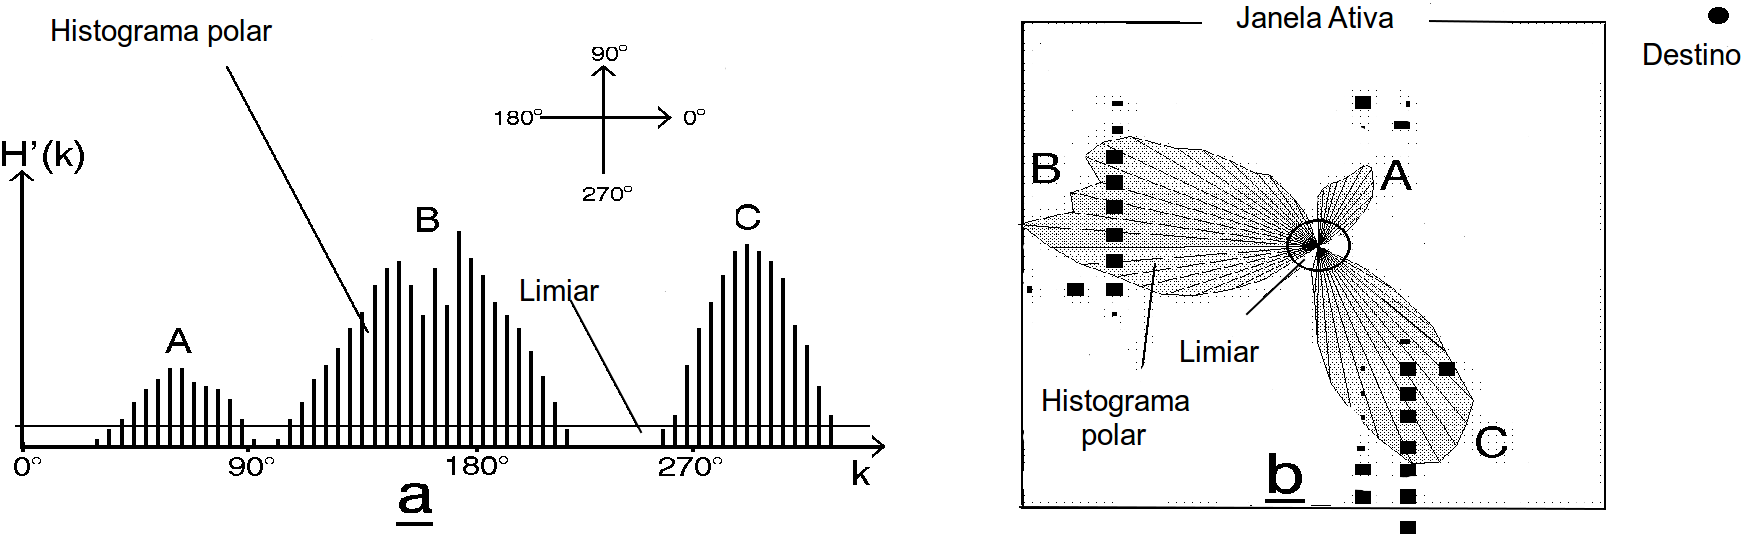
\includegraphics[width=\textwidth,height=7cm]{images/vfh_horiz.png}
	 	\caption{VFH - \textbf{(\underline{a})} Gráfico do histograma, 
	 	onde H'(k) representam as forças de repulsão aos obstáculos nas direções k.\\
	 	\textbf{(\underline{b})} Representação espacial em relação aos 
	 	obstáculos (retângulos em preto) - A área circulada representa a posição do robô.}
		\fonte{adaptado de: \cite{Borenstein1991}}
	 	\label{fig:vfh}
	\end{minipage}
\end{figure}


%Para o planejamento global, de posse de uma mapa convertido em custos 

Enquanto o VFH tem um comportamento mais reativo, em um cenário onde um mapa
global mesmo que incompleto é fornecido pode ser adotado um método deliberativo
para o planejamento da trajetória até um destino.

Os algoritmos de geração de trajetória baseados em amostras tem sido adotado em
robótica móvel com maior ênfase principalmente pela aplicabilidade prática, este
tipo de abordagem leva em consideração a cinemática do veículo gerando
trajetórias realistas com custo computacional baixo \cite{ompl}.

Estes métodos inicialmente constroem um grafo baseado em amostras de trajetórias
que o veículo pode executar, onde geralmente se limita a algumas manobras afim
de reduzir as ramificações do grafo \cite{topologic}. Após esta etapa pode ser
executado um método gráfico de busca por um caminho de menor custo baseado no
menor caminho e proximidade de obstáculos \fig{fig:sbpl}.

\begin{figure}[ht]
	%\hspace{0.1cm}
	\centering
	\begin{minipage}[b]{1\linewidth}
	    \centering
	 	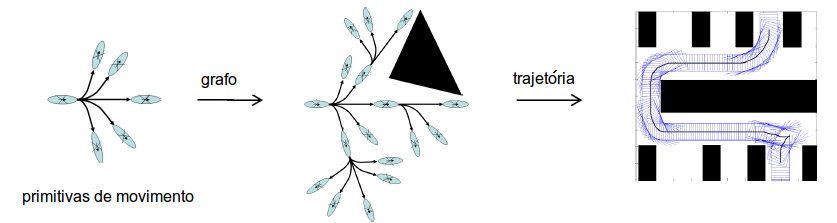
\includegraphics[width=\textwidth,height=5cm]{images/sbpl.png}
	 	\caption{Planejamento de trajetória por amostras}
	 	\fonte{adaptado de: www.ros.org}
	 	\label{fig:sbpl}
	\end{minipage}
\end{figure}
%No trabalho de \cite{} foi utlilizada a biblioteca SBPL
%(\textit{Search-based Planning Library}) 

%Os métodos heurísticos
% baseados em amostra 

\subsection{Controle}

O controle de navegação de um robô móvel pode ser classificado basicamente como
reativo, deliberativo ou híbrido \cite{Wolf2009}, podendo ser estruturada de
forma hierárquica; um caso particular de arquitetura híbrida em camadas. No
projeto COHBRA \cite{Heinen2002}, foi utilizada a abordagem híbrida em camadas
para a criação de um sistema de controle para robôs móveis. Esta abordagem
híbrida permite ao sistema de controle planejar e executar um plano de uma
trajetória (camada deliberativa) ao mesmo tempo em que detecta a presença e
desvia de obstáculos que não foram previamente mapeados (camada reativa). As
técnicas aplicada na elaboração do sistema de controle podem ser baseadas em
Máquinas de Estados Finitos (FSM – \textit{Finite State Machines}), Sistemas
Especialistas e/ou Sistemas Nebulosos (FIS - \textit{Fuzzy Inference Systems}),
Redes Neurais Artificiais (RNA), ou mesmo, uma combinação destes em diversas
camadas. 

As RNAs são consideradas sistemas "caixa-preta": após o treinamento da RNA os
pesos sinápticos associados a cada neurônio (por exemplo, perceptron) não têm
propriamente um “significado”, somente valores numéricos que representam o
conhecimento adquirido. A sua capacidade de generalização torna-a tolerante a
ruídos e permite a aplicação principalmente quando não se consegue estruturar
totalmente o problema a partir de regras bem definidas. É uma técnica
extremamente plástica, podendo ser aplicada a diversas classes de problemas. O
sistema SEVA3D \cite{Heinen2007} se baseou no aprendizado neural de um FSM
(Finite-State Machine) para fazer o controle de navegação do veículo, já no
simulador RoBombeiros \cite{Pessin2008}, adotou-se uma RNA para este fim
(\fig{fig:ann_pesin}).

\vspace{0.5cm}
\begin{figure}[ht]
	%\hspace{0.1cm}
	\centering
	\begin{minipage}[b]{0.6\linewidth}
	    \centering
	 	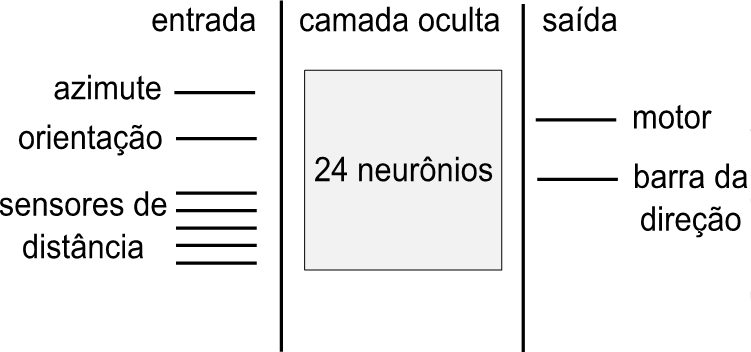
\includegraphics[width=\textwidth,height=5cm]{images/ann_pesin.png}
	 	\caption{Arquitetura da RNA no simulador RoBombeiros}
	 	\label{fig:ann_pesin}
	\end{minipage}
\end{figure}


%OSORIO
%> Podia detalhar um pouco mais sobre o Robombeiros aqui... se não for detalhar
% mais adiante, seria bom ser mais "didático" pois nem todos da banca sabem do
% que se trata e como funciona (assim como os futuros leitores deste texto)

No caso dos RoBombeiros, o controle pela rede neural era de um comportamento
basicamente reativo, onde ao mesmo tempo que direcionava o veículo para o
destino gerava comandos de desvio na presença de obstáculos próximos. Nesta rede
neural foi projetado como entrada a orientação do veículo dada por uma bússola e
a sua orientação em relação ao ponto de destino calculada pelas posições de GPS,
assim como informações sensoriais de distâncias de objetos presentes no raio de
ação do sensor laser utilizado. Desta forma a rede neural foi treinada para
gerar comandos de aceleração e esterçamento que controlavam a navegação do
veículo autônomo.

%2012-10-15 Lido OK
